% article example for classicthesis.sty
\documentclass[10pt,a4paper]{article} % KOMA-Script article scrartcl
\usepackage{import}
\usepackage{xifthen}
\usepackage{pdfpages}
\usepackage{transparent}
\newcommand{\incfig}[1]{%
    \def\svgwidth{\columnwidth}
    \import{./figures/}{#1.pdf_tex}
}
\usepackage{lipsum}     %lorem ipsum text
\usepackage{titlesec}   %Section settings
\usepackage{titling}    %Title settings
\usepackage[margin=10em]{geometry}  %Adjusting margins
\usepackage{setspace}
\usepackage{listings}
\usepackage{amsmath}    %Display equations options
\usepackage{amssymb}    %More symbols
\usepackage{xcolor}     %Color settings
\usepackage{pagecolor}
\usepackage{mdframed}
\usepackage[spanish]{babel}
\usepackage[utf8]{inputenc}
\usepackage{longtable}
\usepackage{multicol}
\usepackage{graphicx}
\graphicspath{ {./Images/} }
\setlength{\columnsep}{1cm}

% ====| color de la pagina y del fondo |==== %



\begin{document}
    %========================{TITLE}====================%
    \title{{  Parcial 3 de algebra abstracta  }}
    \author{{Rodrigo Castillo (junto a Carlos y Oscar)}}
    \date{\today}

    \maketitle


    %=======================NOTES GOES HERE===================%
    \section{Sea c el código lineal de longitud $9$ cuya matriz de control es:}
    \begin{figure}[h!]
        \centering
        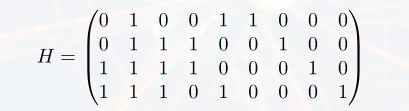
\includegraphics[width=0.8\linewidth]{matrizcontrol.png}
        \caption{matriz de control}
        \label{matriz de control}
    \end{figure}

        \subsection{a : encuentre la dimensión de $C$}
            % ====|ACA EMPIEZA EL PUNTO 1-A|====
        sabemos que si $C$ es un código lineal de longitud $n$ y dimensión $k$
        , una matrix $n-k \times  nH$ es una matriz de control para el código C
        si $wH ^{T} \iff w \in C $
        \\
        sabemos que C tiene longitud $9$
        \\
        $H$ es una matriz $4 \times 9$
        \\
        por lo tanto $n-k = 4$
        \\
        $9-k = 4$
        \\
        $k=5$
        \\
        por lo tanto $dim(C) = 5$

            % ====|ACA TERMINA EL PUNTO 1-A|==== %

        \subsection{encuentre la distancia mínima de $C$}
            % ====|ACA EMPIEZA EL PUNTO 1-b|====
        para este punto necesitamos la matris generadora de $C$ , tenemos que
        $G = (I_k A)$ y que $H = (-A ^{T} I_{n-k})$ luego ...
        \begin{equation}
            G = \begin{pmatrix}
                1 & 0 & 0 & 0 & 0 & 0 & 0 & 1 & 1
                \\
                0 & 1 & 0 & 0 & 0 & 1 & 1 & 1 & 1
                \\
                0 & 0 & 1 & 0 & 0 & 0 & 1 & 1 & 1
                \\
                0 & 0 & 0 & 1 & 0 & 0 & 1 & 1 & 0
                \\
                0 & 0 & 0 & 0 & 1 & 1 & 0 & 0 & 1
            \end{pmatrix}
        \end{equation}
        con $G$ podemos ver que la distancia mínima es $3$
            % ====|ACA TERMINA EL PUNTO 1-b|==== %

        \subsection{calcule los sindromes correspondientes a errores de
            $C$ que puede corregir}
            % ====|ACA EMPIEZA EL PUNTO 1-c|====

            \textbf{sabemos que un código es $e-corrector$ si su distancia
            mínima es $2e +1$ como mínimo} por lo tanto, como la distancia
            mínima de C es 3 , entonces es $1 corrector$ (pues $1+1+1 = 3$ )
            \\
            como el código es $1-corrector$ se tiene que:
            \\
            \textbf{si el síndrome es igual a 0 , no hay error en la palabra}
            \\
            \textbf{si el sindrome $\not= $ 0 , se tiene que la representación
            será un número binario que representa la posición del error}

            % ====|ACA TERMINA EL PUNTO 1-c|==== %

        \subsection{diga si $000110011 \in C$   o no}
            % ====|ACA EMPIEZA EL PUNTO 1-d|====
            lo primero que hicimos fue calcular la matrix $H ^{T} $
            \begin{equation}
                H ^{T} = \begin{pmatrix}
                    0 & 0 & 1 & 1
                    \\
                    1 & 1 & 1 & 1
                    \\
                    0 & 1 & 1 & 1
                    \\
                    0 & 1 & 1 & 0
                    \\
                    1 & 0 & 0 & 1
                    \\
                    1 & 0 & 0 & 0
                    \\
                    0 & 1 & 0 & 0
                    \\
                    0 & 0 & 1 & 0
                    \\
                    0 & 0 & 0 & 1
                \end{pmatrix}
            \end{equation}

            multiplicaremos la palabra por $H ^{T}  $ , si el resultado es
            \textbf{$0000$ significa que la palabra pertenece a $C$}
            \\
            \textbf{$000110011 \cdot H ^{T}  = 1100$ luego tenemos que $000110011
            \notin C$}
            % ====|ACA TERMINA EL PUNTO 1-d|==== %

        \subsection{decodifique $110101101$}
            % ====|ACA EMPIEZA EL PUNTO 1-e|====
            sea la palabra $110101101$ , la multiplicaremos por $H ^{T}  $
            \\
            $110101101 \cdot H ^{T}  = 0111$ , luego el error es $001000000$ ,
            ahora , usando $\omega = c + r $ se tiene que $c = 1111011011$


            % ====|ACA TERMINA EL PUNTO 1-e|==== %
    \section{Punto 2}
    \subsection{sea $g(x)$el generador de un codigo ciclico de longitud
    $15$ sobre $Z_2$ demuestre que $g(1) = 1 \iff $ todas las palabras
    del código tienen un peso par}
        sea $g(x)$ un generador de un código cíclico de longitud $15$ sobre $Z_2$
        \\
        se tiene entonces que $g(x)$ corresponde al ideal de $\langle g(x) \rangle
        $ , luego es un ideal de $ Z_2/\langle X ^{15}  -1 \rangle$ , por lo que
        \\
        $g(x) = c_0 + c_1X + x_2 X ^{2}  + ... + c_{14}X ^{14} $
        \\
        $g(1) = 0$
        \\
        $g(1) = c_0 + c_1X + c_2X ^{2}  + ... + c_{14} X ^{14} = 0 $
        \\
        $g(1) = c_0 + c_1 + c_2 + ... + c_{14} = 0 $
        \\
        como $c_i \in Z_2$  y además $c_i \in C $ entonces $C$ tiene peso par
        \\
        \textbf{la demostración de la otra parte de la equivalencia es análoga}

    \section{Punto 3}
    \subsection{sea F = $\{ 0 , 1 , \omega  , \hat{\omega }  \}$ el campo
    finito con 4 elementos , las operaciones en $F$ siguen de estas reglas...}
        $1+1 = 0$ , $1 + \omega  = \omega ^{2}  = \hat{\omega } $
        \subsubsection{escriba las tablas de operaciones en F}

        % ====|ACA EMPIEZA EL PUNTO 3-a|====

        \begin{figure}[h!]
            \centering
            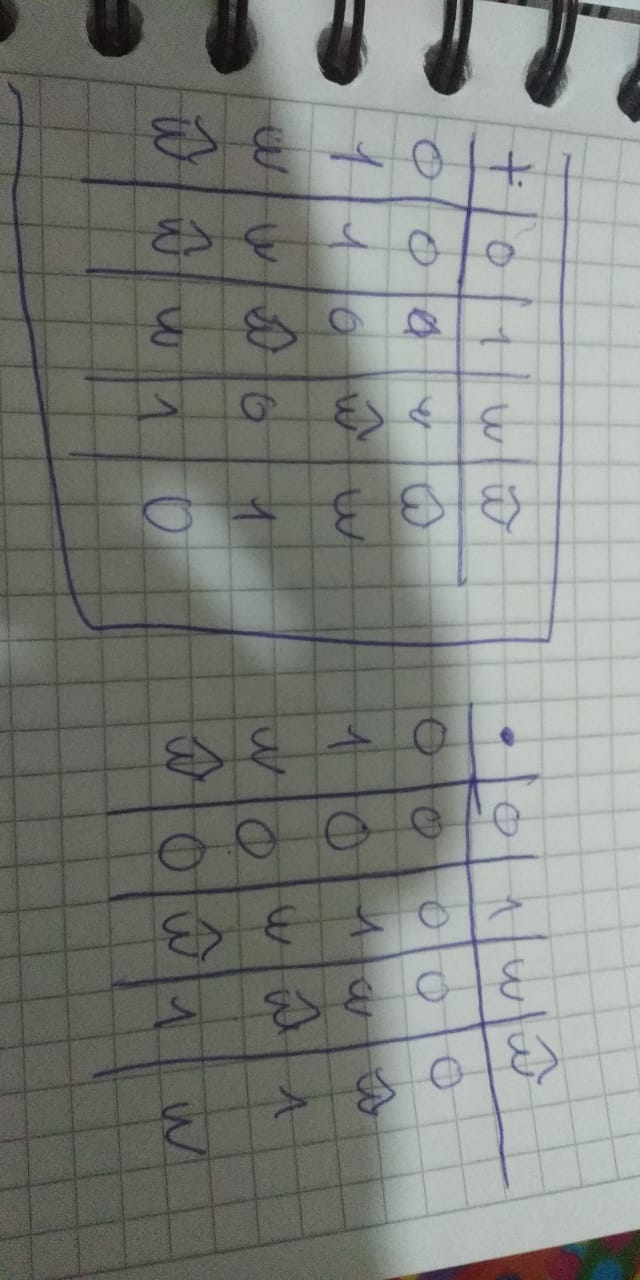
\includegraphics[width=0.4\linewidth , angle = 90]{control.jpeg}
            \caption{tablas de operaciones}
            \label{operaciones}
        \end{figure}
        \color{blue} nota: por alguna razón latex no me dejaba importar la
        libería para hacer una tabla \color{black}


        % ====|ACA TERMINA EL PUNTO 3-a|==== %

        \subsubsection{encuentre el peso minimo de C y una matriz de control para C}
        % ====|ACA EMPIEZA EL PUNTO 3-b|====


        \textbf{el peso mínimo de $G$ es 4}
        \\
       , esto lo sabemos por la distancia mínima
        entre las filas
        \\
        como C es lineal, el peso mínimo de de $C$ es igual al peso mínimo de
        $GJ$ que también es 4
        \\
        $G = (I_k A)$ , $H = -A ^{T} I_{n-k} $ , entonces al hacer $-A ^{T}$
        nos da la matriz ...
        \begin{equation}
            \begin{pmatrix}
                -1 & -1 & -1
                \\
                -1 & -\omega  & -\hat{\omega }
                \\
                -1 & -\hat{\omega}  & -\omega
            \end{pmatrix}
        \end{equation}
        haciendo uso de  la tabla de operacion de la suma podemos saber que $1
        = -1 ,
        \omega  = -\omega $ , podemos decir que  matriz de control    $H$ es :

        \begin{equation}
            H = \begin{pmatrix}
            1 & 1& 1  & 1 & 0 & 0
            \\
            1 & \omega & \hat{\omega }   & 0 & 1 & 0
            \\
            1 & \hat{omega} & \omega   & 0 & 0 & 1
            \end{pmatrix}
        \end{equation}

        \subsubsection{demuestre que ningun codigo sobre un alfabeto de 4
        simbolos con la misma longitud y distancia mínima de C puede tener mas
        palabras códigos que C}
            C tiene 64 palabras, luego
            \\
            \textbf{sabemos que C cumple la cota del singulete} , luego $|C| <= 4 ^{3} $
            luego $C <= 64$ luego no hay un código que sea tenga mas palabras
            códigos que C(pues $C$ tiene 64 palabras)


        % ====|ACA TERMINA EL PUNTO 3-b|==== %

        \section{PUNTO 4}
            % ====|ACA EMPIEZA EL PUNTO 4|====

            sea H una matriz de control para el código lineal C sobre $Z_2$ de
            longitud n y dimension k, construimos un nuevo código $C'$ de
            longitud $n+1$ en la siguiente manera:
            si $c_0c_1...c_{n-1} \in C$ entonces $c_0c_1 ... c_{n-1}c_n \in C'$
            con $c_n = c_0 + c_1 + ... + c_{n-1}$

            \textbf{Encuentre la dimensión, distancia minima y matriz de
            control de C' en función de los mismos para C}
            \\
            como C' es C mas la añadidura de un simbolo a la longitud sabemos
            que la dimensión de C es k
            \\
            Sabemos por teorema dado en clase que \textbf{el peso minimo de un
            codigo lineal es su distancia minima} , por lo que en el caso de
            este ejercicio se tiene que  ...
            \\
            si el peso de C es par , como C tiene una cantidad par de $1's y
            c_n$ es la suma del código añadimos un 0. dandonos cuenta de que
            esto no afecta el peso de C' por que si el peso de C es par, la
            distancia minima de C' será igual a la de C
            \\
            si el peso de C es impar en , sumamos una cantidad impar de $1's$ ,
            entonces añadiremos un 1 a la suma de $c_n$ , por lo que la
            distancia minima de $C'$ cuando C es impar , la distancia mínima es
            $C+1$
            \\
            \textbf{Matriz de control} :
            \\
            Sabemos que $(C_0 ... C_{n-1} H ^{T}  = 0 )$ , por lo tanto $C_0
            ... C_n \in C'$, además , $c_n = c_0 + c_1 + ... + c_{n-1} $
            \\
            tenemos que $C'  H' ^{T} $ debe ser igual a 0 , por lo que
            debemos lograr que al agregarle la matriz $H$ siga cumpliendo la
            igualdad.
            \\
            para esto tomaremos $H ^{T} $ y le agregaremos una columna de $1's$
            al final
            \\
            luego una fila de $0's$ al final hasta la posición $nXn-1$
            de manera que la entrada  $nXn$ sea un 1 también
            \\
            al momento de
            hacer la transpuesta de esta nueva matriz generaremos a $H'$ ,
            matriz en la
            cuál las primeras filas y columnas serán iguales a las de $H$ y a
            la ultima columna serán $0's$ hasta la posición $n-1Xn$ y la ultima
            fila será $0s$ teniendo así en la posición $nXn$ un 1 .
            De esta manera generaremos una matriz $H$ que al multiplicarla con
            la matriz descrita arriba, obtendremos $0$ y por lo tanto esta
            matriz será una matriz de control para el código $C$


            % ====|ACA TERMINA EL PUNTO 4|==== %























    %=======================NOTES ENDS HERE===================%

    % bib stuff
    \nocite{*}
    \addtocontents{toc}{{}}
    \addcontentsline{toc}{section}{\refname}
    \bibliographystyle{plain}
    \bibliography{../Bibliography}
\end{document}
